\documentclass{report}
\usepackage[utf8]{inputenc}
\usepackage[spanish]{babel}
\usepackage[T1]{fontenc}

\usepackage{amsmath,amsfonts,amsthm,amssymb}
\usepackage{setspace}
\usepackage{Tabbing}
\usepackage{fancyhdr}
\usepackage{lastpage}
\usepackage{extramarks}
\usepackage{chngpage}
\usepackage{soul,color}
\usepackage{graphicx,float,wrapfig}
\usepackage{graphicx}
\usepackage{listings}
\usepackage{color}
\usepackage{multirow}

% Some configurations
\graphicspath{ {images/} }
\lstset {language=C++}

% In case you need to adjust margins:
\topmargin=-0.45in      %
\evensidemargin=0in     %
\oddsidemargin=0in      %
\textwidth=6.5in        %
\textheight=9.0in       %
\headsep=0.25in         %

% Homework Specific Information
\newcommand{\tpTitle}{TP\ 1 - Scheduling}
\newcommand{\materia}{SO}

% Setup the header and footer
\pagestyle{fancy}                                    %  
\fancyhead{}                                         % Remove all header contents
\renewcommand{\headrulewidth}{0pt}                   % Remove header line
\lfoot{\lastxmark}                                   %
\cfoot{}                                             %
\rfoot{Page\ \thepage\ of\ \pageref{LastPage}}       %
\renewcommand\footrulewidth{0.4pt}                   %

%%%%%%%%%%%%%%%%%%%%%%%%%%%%%%%%%%%%%%%%%%%%%%%%%%%%%%%%%%%%%
% Some tools
\newcommand{\enterProblemHeader}[1]{\nobreak\extramarks{#1}{#1 continuado en la próxima página\ldots}\nobreak%
                                    \nobreak\extramarks{#1 (continued)}{#1 continuado en la próxima página\ldots}\nobreak}%
\newcommand{\exitProblemHeader}[1]{\nobreak\extramarks{#1 (continued)}{#1 continuado en la próxima página\ldots}\nobreak%
                                   \nobreak\extramarks{#1}{}\nobreak}%

\newlength{\labelLength}
\newcommand{\labelAnswer}[2]
  {\settowidth{\labelLength}{#1}%
   \addtolength{\labelLength}{0.25in}%
   \changetext{}{-\labelLength}{}{}{}%
   \noindent\fbox{\begin{minipage}[c]{\columnwidth}#2\end{minipage}}%
   \marginpar{\fbox{#1}}%

   % We put the blank space above in order to make sure this
   % \marginpar gets correctly placed.
   \changetext{}{+\labelLength}{}{}{}}%

\setcounter{secnumdepth}{0}
\newcommand{\homeworkProblemName}{}%
\newcounter{homeworkProblemCounter}%
\newenvironment{homeworkProblem}[1][Problem \arabic{homeworkProblemCounter}]%
  {\stepcounter{homeworkProblemCounter}%
   \renewcommand{\homeworkProblemName}{#1}%
   \section{\homeworkProblemName}%
   \enterProblemHeader{\homeworkProblemName}}%
  {\exitProblemHeader{\homeworkProblemName}}%

\newcommand{\problemAnswer}[1]
  {\noindent\fbox{\begin{minipage}[c]{\columnwidth}#1\end{minipage}}}%

\newcommand{\problemLAnswer}[1]
  {\labelAnswer{\homeworkProblemName}{#1}}

\newcommand{\homeworkSectionName}{}%
\newlength{\homeworkSectionLabelLength}{}%
\newenvironment{homeworkSection}[1]%
  {% We put this space here to make sure we're not connected to the above.
   % Otherwise the changetext can do funny things to the other margin

   \renewcommand{\homeworkSectionName}{#1}%
   \settowidth{\homeworkSectionLabelLength}{\homeworkSectionName}%
   \addtolength{\homeworkSectionLabelLength}{0.25in}%
   \changetext{}{-\homeworkSectionLabelLength}{}{}{}%
   \subsection{\homeworkSectionName}%
   \enterProblemHeader{\homeworkProblemName\ [\homeworkSectionName]}}%
  {\enterProblemHeader{\homeworkProblemName}%

   % We put the blank space above in order to make sure this margin
   % change doesn't happen too soon (otherwise \sectionAnswer's can
   % get ugly about their \marginpar placement.
   \changetext{}{+\homeworkSectionLabelLength}{}{}{}}%

\newcommand{\sectionAnswer}[1]
  {% We put this space here to make sure we're disconnected from the previous
   % passage

   \noindent\fbox{\begin{minipage}[c]{\columnwidth}#1\end{minipage}}%
   \enterProblemHeader{\homeworkProblemName}\exitProblemHeader{\homeworkProblemName}%
   \marginpar{\fbox{\homeworkSectionName}}%

   % We put the blank space above in order to make sure this
   % \marginpar gets correctly placed.
   }%

%%%%%%%%%%%%%%%%%%%%%%%%%%%%%%%%%%%%%%%%%%%%%%%%%%%%%%%%%%%%%


%%%%%%%%%%%%%%%%%%%%%%%%%%%%%%%%%%%%%%%%%%%%%%%%%%%%%%%%%%%%%
% Make title
\title{\vspace{2in}\textmd{\textbf{\materia:\ \tpTitle}}}
\date{}
\author{
  Andreas Sturmer\\
  \texttt{remruts@gmail.com}
  \and
  Dan Zajdband\\
  \texttt{dan.zajdband@gmail.com}
  \and
  Javier Casal\\
  \texttt{javierjcasal@gmail.com}
}
%%%%%%%%%%%%%%%%%%%%%%%%%%%%%%%%%%%%%%%%%%%%%%%%%%%%%%%%%%%%%

\begin{document}
\begin{spacing}{1.3}
\maketitle
\newpage
% Uncomment the \setcounter line as well if you do NOT want subsections
%       listed in Contents
\tableofcontents
\newpage

\clearpage
\begin{homeworkProblem}[Ejercicio 1]
    En este primer ejercicio se nos pide programar una tarea interactiva que realice  \textit{n} llamadas bloqueantes de una duraci\'on al azar comprendida entre dos de los par\'ametros que la tarea recibe (el tercer par\'ametro es \textit{n}, es decir, la mencionada cantidad de llamadas bloqueantes).\\

\textbf{Implementaci\'on} \\
        Para ello empezamos por registrar la tarea en la funci\'on provista \textit{tasks\_init} seg\'un se indica. Luego implementamos la funci\'on reci\'en registrada vali\'endonos de la funci\'on \textit{uso\_IO} que resulta en una llamada bloqueante de \textit{t} ciclos de reloj en completar (donde \textit{t} es el \'unico par\'ametro que \textit{uso\_IO} recibe. Falta \'unicamente mencionar que, para definir un tiempo al azar que est\'e comprendido entre los valores solicitados, realizamos una suma que adicione el m\'inimo necesario a un valor aleatroio comprendido entre la diferencia entre el m\'inimo (\textit{bmin}) y el m\'aximo (\textit{bmax}) recibidos:
            \begin{center}
            bmin + (rand() \% ((bmax + 1) - bmin))
            \end{center} 

\textbf{Gr\'afico de un lote de tareas} \\
        El gr\'afico a continuaci\'on (\textit{Figure 1}) corresponde a un lote de 1 tarea que realiza 4 llamadas bloqueantes de entre 2 y 7 tiempos de duraci\'on: \\
        \begin{figure}[h]
            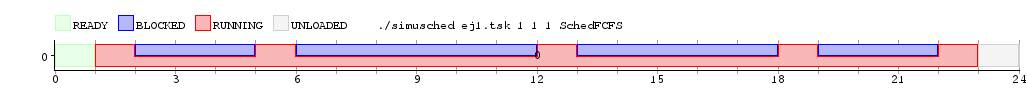
\includegraphics[width=1\textwidth]{ej1}
            \caption{}
        \end{figure} \\
No son muchas las cosas a revisar, entre ellas: \\
- Las llamadas bloqueantes son, en efecto, 4 \\
- Las llamadas bloqueantes en ning\'un caso duran menos de 2 tiempos \\
- Las llamadas bloqueantes en ning\'un caso se exceden de 7 tiempos de duraci\'on

\end{homeworkProblem}

\clearpage
\begin{homeworkProblem}[Ejercicio 2]
    En este segundo ejercicio estamos a cargo de Rolando, su complejo algoritmo, y sus distracciones al momento de sentarse a la computadora. \\
    Nuestro primer encargo es escribir un lote de tareas que simule la situaci\'on de Rolando descripta en el enunciado. Este lote incluye entonces una primer corrida de 100 ciclos de CPU en ning\'un caso bloqueantes buscando simular los 100 ciclos de corrida del algoritmo complejo de Rolando. Nos valemos para ello de la funci\'on provista \textit{TaskCPU}. Lo siguiente ser\'an 2 tareas con llamadas bloqueantes de una duraci\'on variable dentro de un rango; en otras palabras, 2 tareas que realizan exactamente aquello que se nos pidi\'o en el primer ejecicio del trabajo pr\'actico. Usamos entonces la tarea \textit{TaskConsola} con los par\'ametros correspondientes para simular las tareas de ocio de Rolando. \\
    
    \textbf{Gr\'aficos utilizando 1 y 2 n\'ucleos} \\
    Los gr\'aficos a continuaci\'on (\textit{Figure 2}) corresponden a la ejecuci\'on de la simulaci\'on utilizando el algoritmo FCFS para 1 core (Figure 2) y para 2 cores (Figure 3). En ambos casos el costo de cambio de contexto es de 4 ciclos.
    
    \begin{figure}[h]
        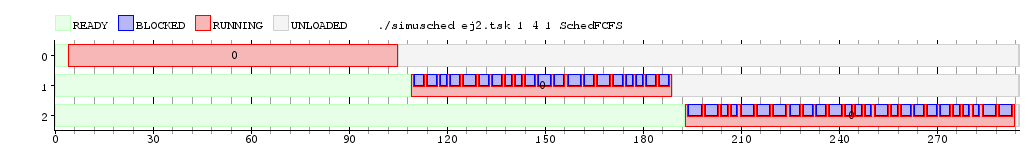
\includegraphics[width=1\textwidth]{ej2-1core}
        \caption{}
    \end{figure}
    
    \begin{figure}[h]
        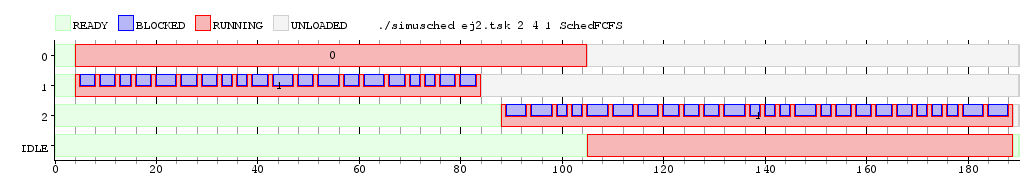
\includegraphics[width=1\textwidth]{ej2-2core}
        \caption{}
    \end{figure}

    \textbf{Latencia} \\
    La siguiente asignatura es el c\'alculo de la latencia de cada una de las tareas en cada uno de los dos casos:
\begin{table}[h]
  \begin{center}
\begin{tabular}{c|c|c|c}
        & Tarea 1 & Tarea 2 & Tarea 3 \\
\hline
1 core  & 4       & 109     & 193     \\
\hline
2 cores & 4       & 4       & 88     
\end{tabular}
  \end{center}
\end{table}
    
    
\end{homeworkProblem}

\clearpage
\begin{homeworkProblem}[Ejercicio 3]
    Work in progress...
\end{homeworkProblem}

\clearpage
\begin{homeworkProblem}[Ejercicio 4]
    Work in progress...
\end{homeworkProblem}

\clearpage
\begin{homeworkProblem}[Ejercicio 5]
    Work in progress...
\end{homeworkProblem}

\clearpage
\begin{homeworkProblem}[Ejercicio 6]
    Work in progress...
\end{homeworkProblem}

\clearpage
\begin{homeworkProblem}[Ejercicio 7]
    Work in progress...
\end{homeworkProblem}

\clearpage
\begin{homeworkProblem}[Ejercicio 8]
    Work in progress...
    En este punto, se nos asignó la tarea de implementación de un scheduler Round-Robin que no permita la migración de procesos
entre núcleos. La asignación de CPU se realizaría en el momento de carga de un proceso y el núcleo correspondiente al mismo sería aquel con menor cantidad de procesos activos totales.

\bigskip

\textbf{Implementación}

La implementación de este scheduler no difiere mucho del de la del ejercicio 4, sólo que en este caso se tiene una cola de procesos por CPU. Además, se posee un entero por CPU (en un vector) que indica la cantidad de procesos activos para cada uno de estos, a ser utilizados cuando se cargue un proceso nuevo. Por último, poseemos un mapa de procesos para saber a qué CPU corresponde cada uno.

Al cargar un proceso, se obtiene el índice (CPU) del mínimo elemento del vector de "activos" y con eso se empuja el proceso a la cola correspondiente y se aumenta la cantidad de activos. Por último, se agrega el proceso con su CPU al mapa de procesos.

Al hacer un tick, la única diferencia con el código del ejercicio 4, además de elegir la cola correspondiente al cpu indicado, es al momento de finalización de una tarea. En este caso, se le resta uno a la cantidad de activos del CPU y se elimina al proceso del mapa de procesos. Luego, es análogo.

Al desbloquearse un proceso, simplemente se obtiene el CPU del mismo a través del mapa de procesos. Con esto, se empuja al proceso al core correspondiente.

\bigskip

\textbf{Ejemplo 1}

Un escenario en el que este scheduler es peor en contraposición con el Round-Robin tradicional, es cuando se van alternando procesos de corta duración con procesos que tarden bastante, como por ejemplo sería el caso de INSERTE EJEMPLO DE LA VIDA REAL AQUÍ. En este caso, terminarían primero los procesos de corta duración, quedando CPUs sin ningún proceso asignado; no se estarían utilizando, realentizando el tiempo de compleción de los procesos y probablemente su tiempo de espera. Sin embargo, la latencia no se vería afectada y sería la misma en ambos casos.

Para ejemplificar esto, construimos un lote de 7 tareas "TaskCPU", alternadas en tiempos de 1 y 8 ciclos. A continuación, se presenta un gráfico de tal lote que simula la situación planteada:

\begin{figure}[h]
    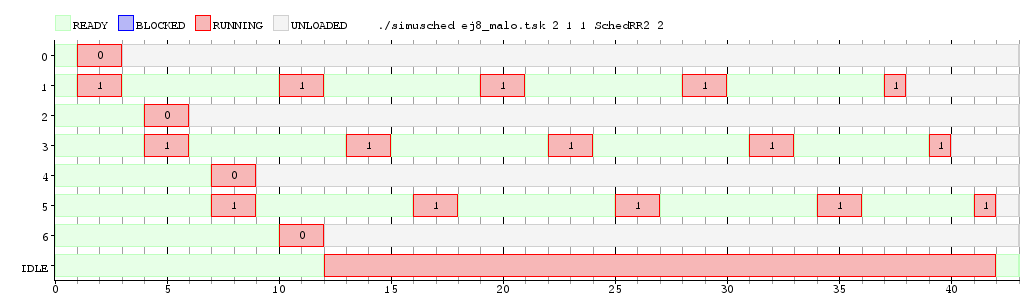
\includegraphics[width=1\textwidth]{ej8MaloRR2}
    \caption{Ejecución en Round-Robin 2}
    \label{RR2Malo}
\end{figure}

Como se muestra en la figura \ref{RR2Malo}, podemos notar lo antes mencionado. Con este nuevo scheduler, a partir del instante 16, el CPU 0, ya no posee ninguna tarea a ejecutar, siendo que terminaron todas las que fueron asignadas al mismo al momento de carga. Por lo tanto, queda en IDLE, mientras que el CPU 1 ejecuta alternadamente los 3 procesos restantes.

En la siguiente tabla mostramos distintas métricas, correspondientes a esta simulación:
% Tabla RR2
\begin{table}[h]
  \caption{Ejecución en Round-Robin 2}
  \centering
    \begin{tabular}{c c c c c}
    \hline
          & Latencia & Espera & Compleción & Ratio (E/C) \\
    \hline
        0 &     1    &    1   &      3     &     0.333   \\
        1 &     1    &   29   &     38     &     0,763   \\
        2 &     4    &    4   &      6     &     0.666   \\
        3 &     4    &   31   &     40     &     0.775   \\
        4 &     7    &    7   &      9     &     0.777   \\
        5 &     7    &   33   &     42     &     0,785   \\
        6 &     10   &   10   &     12     &     0.833   \\
        AVG & 4,857  & 16,428 &   21,428   &     0,705   \\
    \end{tabular}
\end{table}


En cambio, en la figura \ref{RRMalo} (que se presenta a continuación), podemos observar, como con el Round-Robin tradicional, cuando terminan de ejecutarse las tareas cortas (0, 2, 4 y 6), el CPU 1 sigue siendo utilizado por las restantes. Notar que aunque perdemos 1 ciclo extra por cada cambio de CPU, los procesos siguen terminando antes que con el nuevo scheduler implementado.

\begin{figure}[h]
    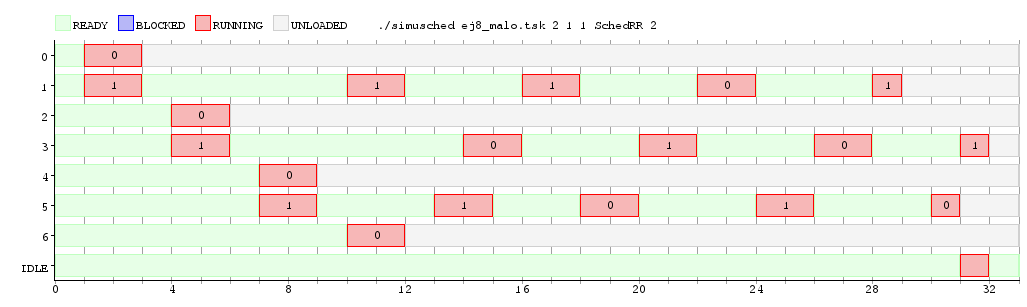
\includegraphics[width=1\textwidth]{ej8MaloRR}
    \caption{Ejecución en Round-Robin Tradicional}
    \label{RRMalo}
\end{figure}

En la siguiente tabla volcamos datos con las mismas métricas que en la tabla correspondiente a \textit{Round-Robin 2}.

% Tabla RR1
\begin{table}[h]
  %\captionsetup{justification=justified,singlelinecheck=false}
  \caption{Ejecución en Round-Robin Tradicional}
  \centering
    \begin{tabular}{c c c c c}
    \hline
          & Latencia & Espera & Compleción & Ratio (E/C) \\
    \hline
        0 &     1    &    1   &      3     &    0.333    \\
        1 &     1    &   20   &     29     &    0,690    \\
        2 &     4    &    4   &      6     &    0.666    \\
        3 &     4    &   23   &     32     &    0,719    \\
        4 &     7    &    7   &      9     &    0.777    \\
        5 &     7    &   22   &     31     &    0,710    \\
        6 &     10   &   10   &     12     &    0.833    \\
        AVG & 4,857  & 12,429 &   17,428   &    0,675    \\
    \end{tabular}
\end{table}

Como supusimos anteriormente, podemos ver como el tiempo de espera y compleción de los procesos largos es menor en \textit{Round-Robin Tradicional}, por lo que en promedio también es mejor. La latencia se mantiene estable.

\bigskip

\textbf{Ejemplo 2}

Sin embargo, este nuevo tipo de scheduler resulta útil en algunas situaciones. Tal es el caso cuando se quisiera lanzar un proceso que ejecute en tiempo real. A modo ilustrativo, en el ejemplo anterior, podría el usuario querer ejecutar alguna especie de simulación de física. Imaginemos que ya se terminaron de ejecutar los procesos cortos y queda un core libre. Entonces, la simulación correría sin interrupciones, y aunque llegaran más procesos, en principio caerían probablemente  en el mismo CPU (si los otros procesos no terminaron), pero estaría balanceado. El tiempo de espera sería menor, como probablemente también la latencia de la simulación.

Para reflejar este comportamiento, modificamos el lote de tareas anterior, agregando la tarea 7 (TaskCPU de 12 ciclos) en el momento 4. Además, agregamos dos tareas pequeñas más que interrumpen a la tarea 7. El gráfico correspondiente se encuentra a continuación:

\begin{figure}[h]
    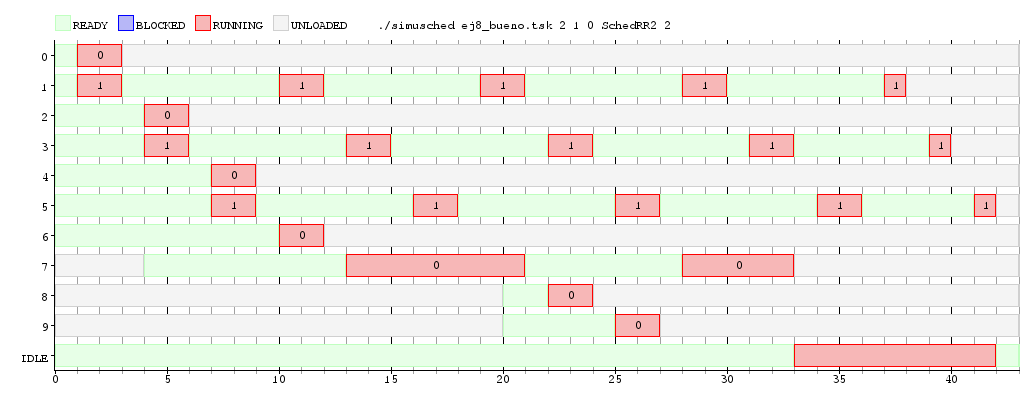
\includegraphics[width=1\textwidth]{ej8BuenoRR2}
    \caption{Ejecución en Round-Robin 2}
    \label{RR2Bueno}
\end{figure}

Como mencionamos, si bien la tarea 7 es interrumpida, tiene un corto tiempo de espera (7 ciclos). Compararlo con la figura \ref{RR2Malo} que se presenta a continuación:

\begin{figure}[h]
    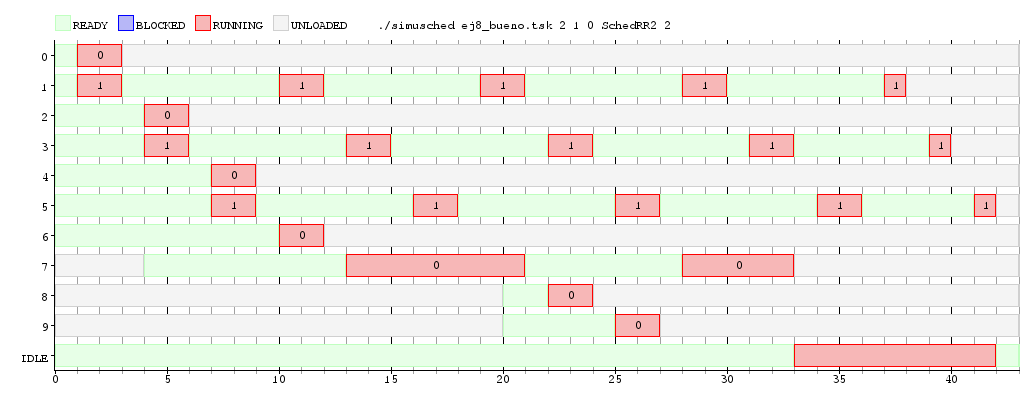
\includegraphics[width=1\textwidth]{ej8BuenoRR2}
    \caption{Ejecución en Round-Robin Tradicional}
    \label{RR2Malo}
\end{figure}

Si bien la tarea 7 tiene la misma latencia en ambos casos, el tiempo de espera es mucho mayor en el \textit{Round-Robin Tradicional}. Como sólo nos importa esta tarea realmente, presentamos una tabla comparativa entre ambos Schedulers para la tarea 7.

\begin{table}[h]
  \caption{Comparación entre schedulers para la tarea 7}
  \centering
    \begin{tabular}{c c c c c}
    \hline
            & Latencia & Espera & Compleción & Ratio (E/C) \\
    \hline
        RR  &     1    &   15   &     28     &    0.536    \\
        RR2 &     1    &    7   &     20     &    0.35     \\
    \end{tabular}
\end{table}

Notar que si no existieran las tareas 8 y 9 que interrumpen ó si hubiera un core libre, la espera sería 0. Igualmente, es notable la mejora que provee el nuevo scheduler en esta situación particular.

Además de esto, en la realidad hay otros factores a considerar que no podrían ser medidos con la simulación utilizada. Por ejemplo, en arquitecturas SMP, es importante mantener cierta afinidad al procesador asignado al proceso, para aprovechar la caché. Si hubiera cambio de procesador, el proceso llegaría con la caché vacía, produciéndose un miss y teniendo que ir a buscar los datos a memoria principal. A esto se le suma el tiempo de los cambios de procesador y de contexto que no son despreciables. En ese sentido, el nuevo scheduler sería preferible al \textit{Round-Robin Tradicional}.

\end{homeworkProblem}


\end{spacing}
\end{document}

%%%%%%%%%%%%%%%%%%%%%%%%%%%%%%%%%%%%%%%%%%%%%%%%%%%%%%%%%%%%%

%----------------------------------------------------------------------%
% The following is copyright and licensing information for
% redistribution of this LaTeX source code; it also includes a liability
% statement. If this source code is not being redistributed to others,
% it may be omitted. It has no effect on the function of the above code.
%----------------------------------------------------------------------%
% Copyright (c) 2007, 2008, 2009, 2010, 2011 by Theodore P. Pavlic
%
% Unless otherwise expressly stated, this work is licensed under the
% Creative Commons Attribution-Noncommercial 3.0 United States License. To
% view a copy of this license, visit
% http://creativecommons.org/licenses/by-nc/3.0/us/ or send a letter to
% Creative Commons, 171 Second Street, Suite 300, San Francisco,
% California, 94105, USA.
%
% THE SOFTWARE IS PROVIDED "AS IS", WITHOUT WARRANTY OF ANY KIND, EXPRESS
% OR IMPLIED, INCLUDING BUT NOT LIMITED TO THE WARRANTIES OF
% MERCHANTABILITY, FITNESS FOR A PARTICULAR PURPOSE AND NONINFRINGEMENT.
% IN NO EVENT SHALL THE AUTHORS OR COPYRIGHT HOLDERS BE LIABLE FOR ANY
% CLAIM, DAMAGES OR OTHER LIABILITY, WHETHER IN AN ACTION OF CONTRACT,
% TORT OR OTHERWISE, ARISING FROM, OUT OF OR IN CONNECTION WITH THE
% SOFTWARE OR THE USE OR OTHER DEALINGS IN THE SOFTWARE.
%----------------------------------------------------------------------%
